\documentclass{article}

\usepackage{graphicx}
\usepackage{tikz}
\usetikzlibrary{calc, spy}
\usepackage{adjustbox}
\usepackage[tightpage, active, floats, graphics]{preview}

\begin{document}
\begin{preview}
    \begin{tikzpicture}
        \begin{scope}[spy using outlines={blue, circle, line width=3pt,
                magnification=6, size=60, connect spies}]
                \node {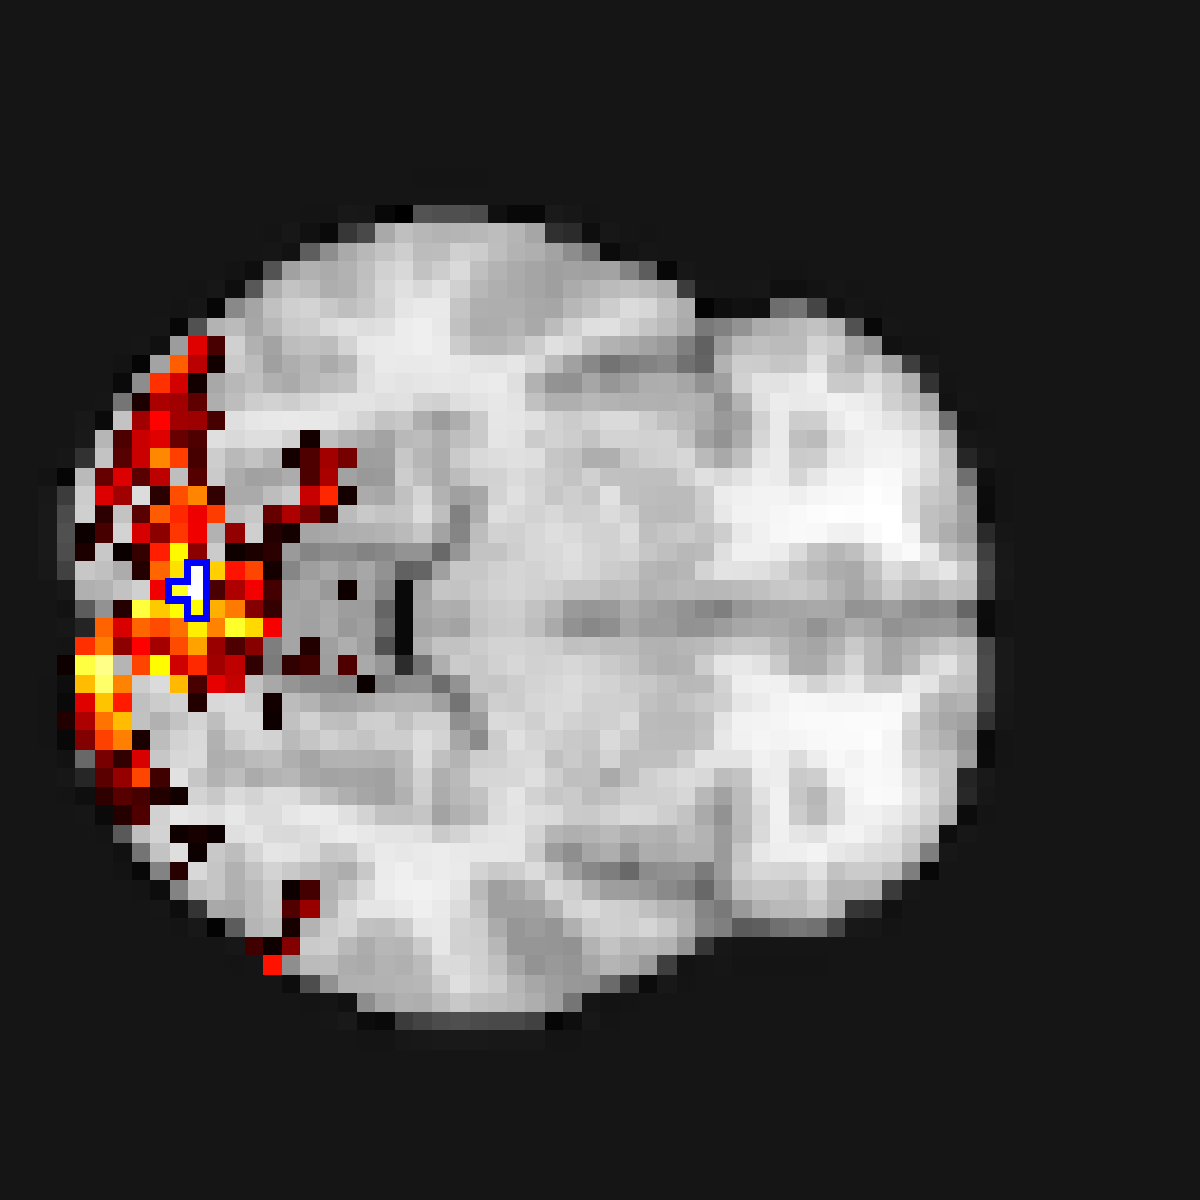
\includegraphics[width=5cm]{encoding_scores}};
            \spy [width=3cm, height=3cm, line width=3pt, spy connection path={\draw[line
            width=2pt, blue] (tikzspyonnode) -- (tikzspyinnode);}]
            on (-0.04, -1.7) in node (a) [line width=4pt] (a) at (1.2,1) (a) {};
        \end{scope} 

        \node (legend) at (4.4, -0.3) {\textsf{Receiptive fields}};
        \node (colorbar) at (4.4, -0.9)
        {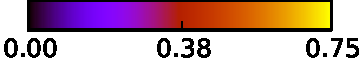
\includegraphics[width=2.4cm]{rf_colorbar}};
        
        \node (i1780) at (4.4, 1.3)
            {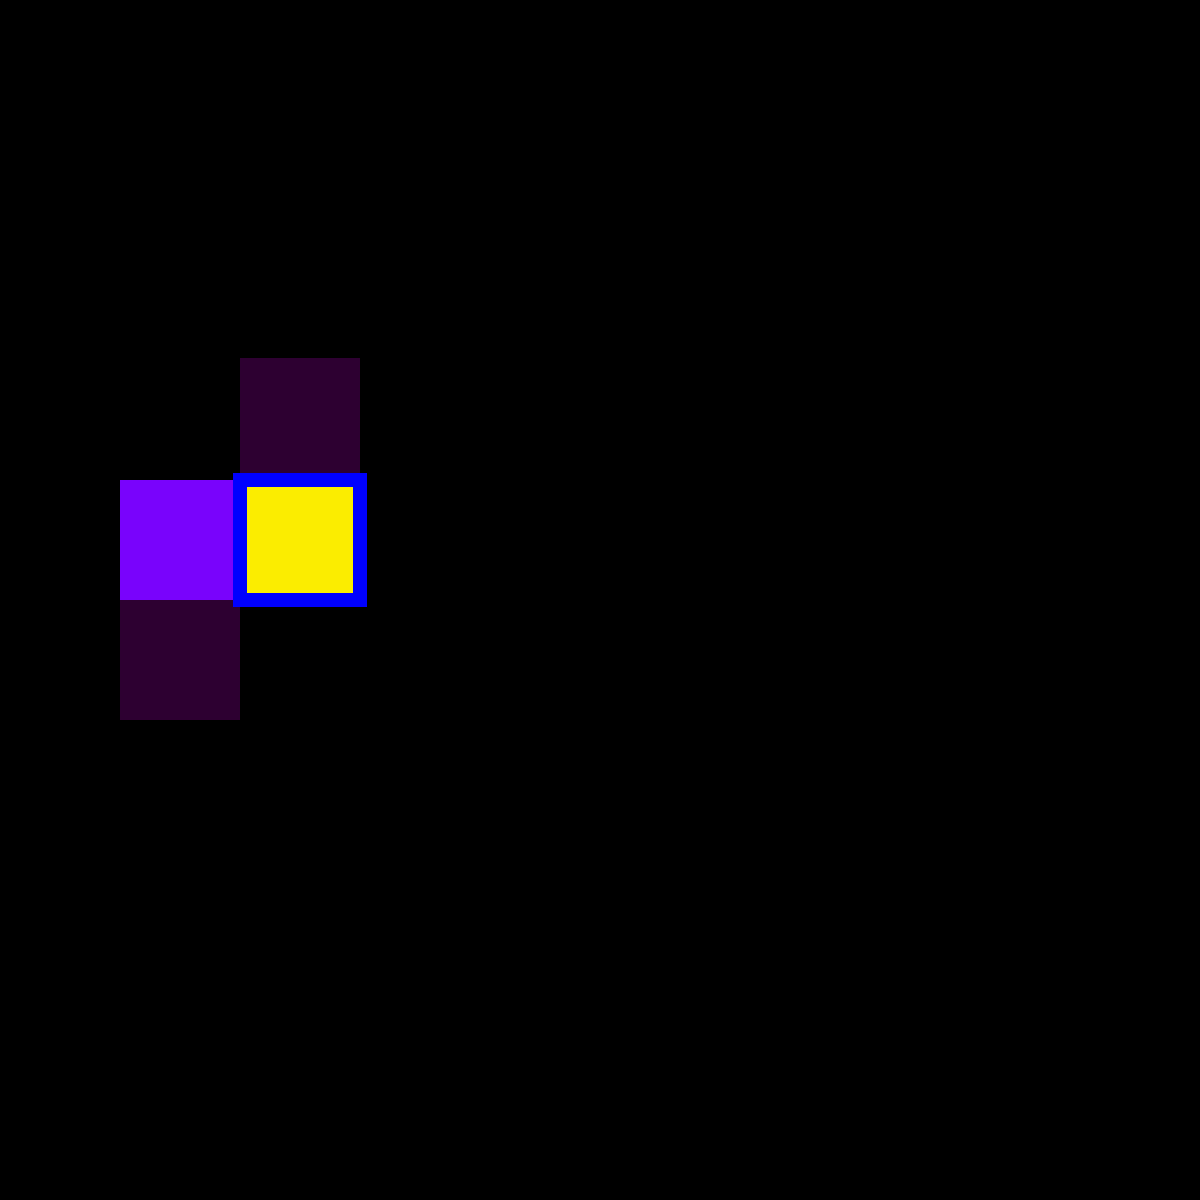
\includegraphics[width=2.4cm]{encoding_1780}};
        \node (i1951) at (7, 1.3)
            {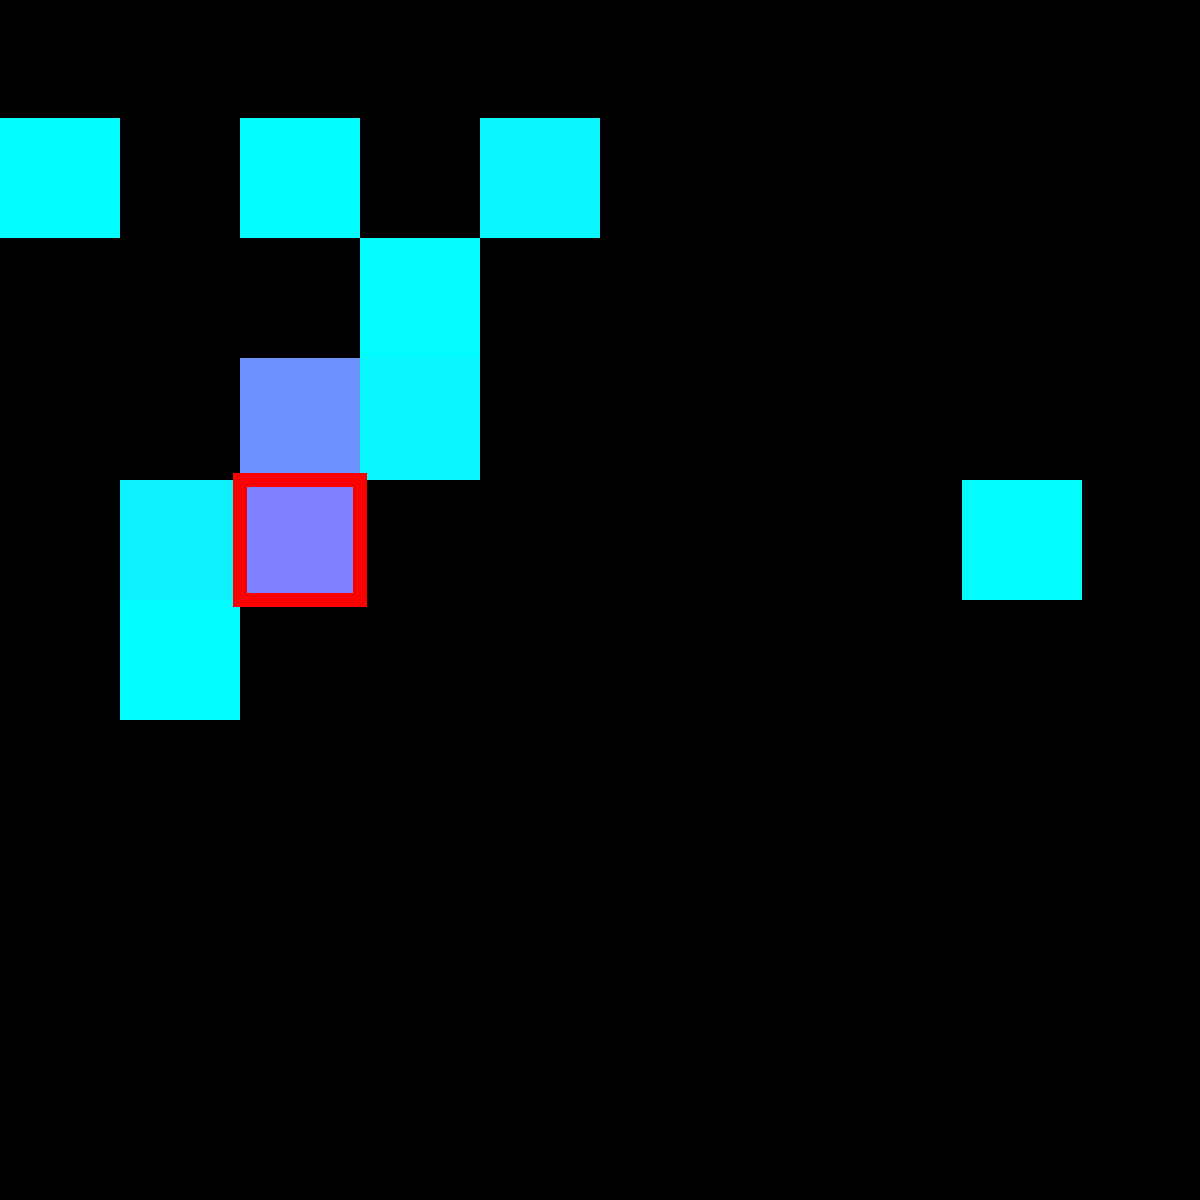
\includegraphics[width=2.4cm]{encoding_1951}};
        \node (i2131) at (9.6, 1.3)
            {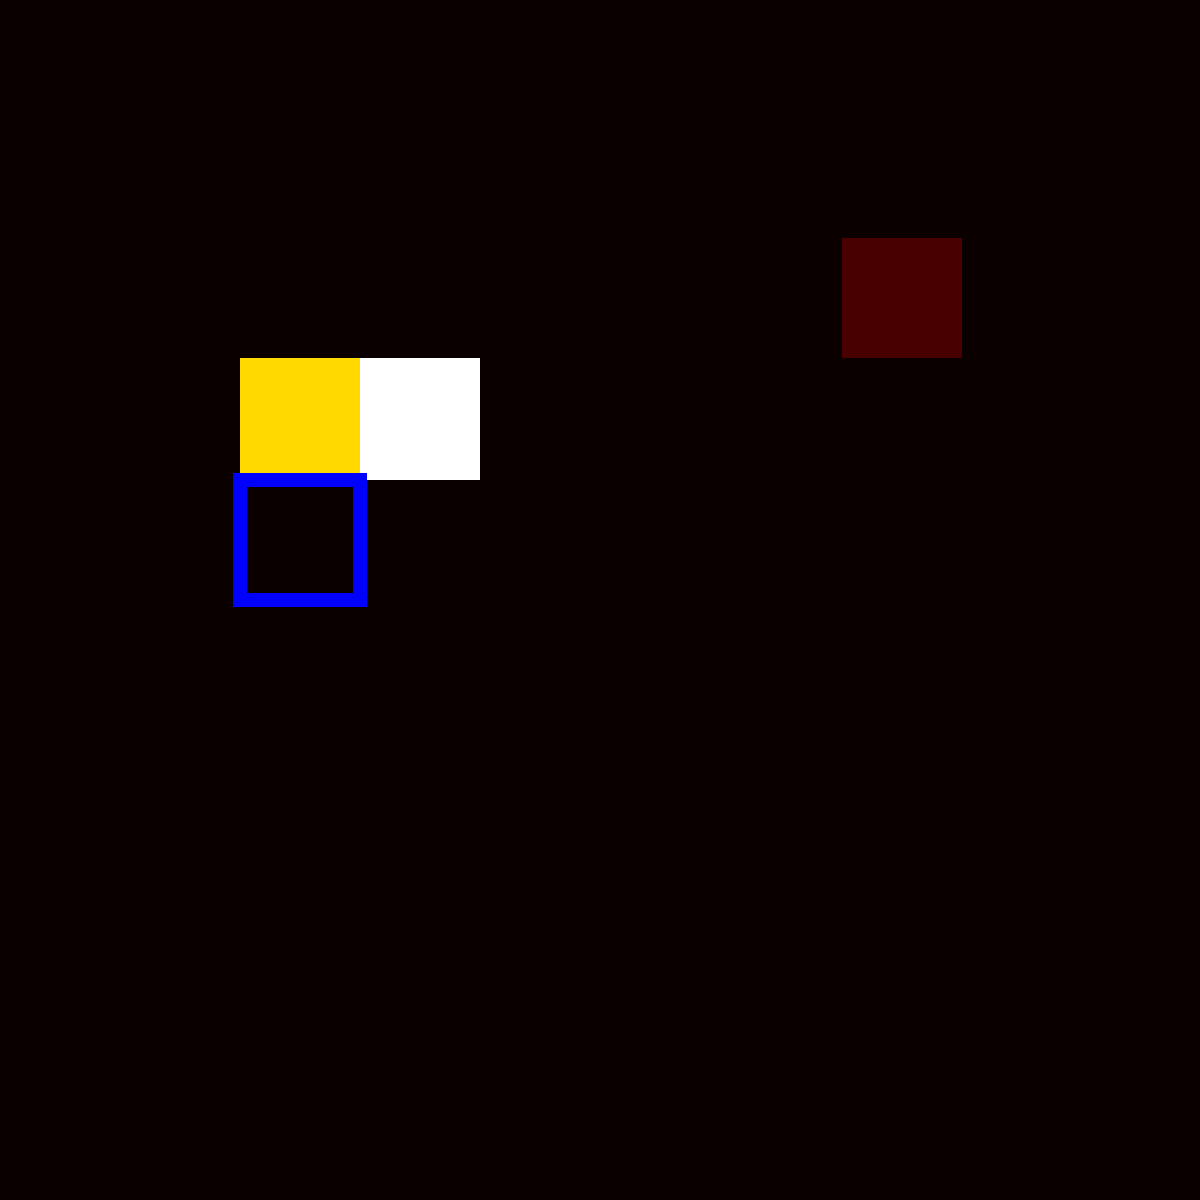
\includegraphics[width=2.4cm]{encoding_2131}};
        \node (i1935) at (7, -1.3)
            {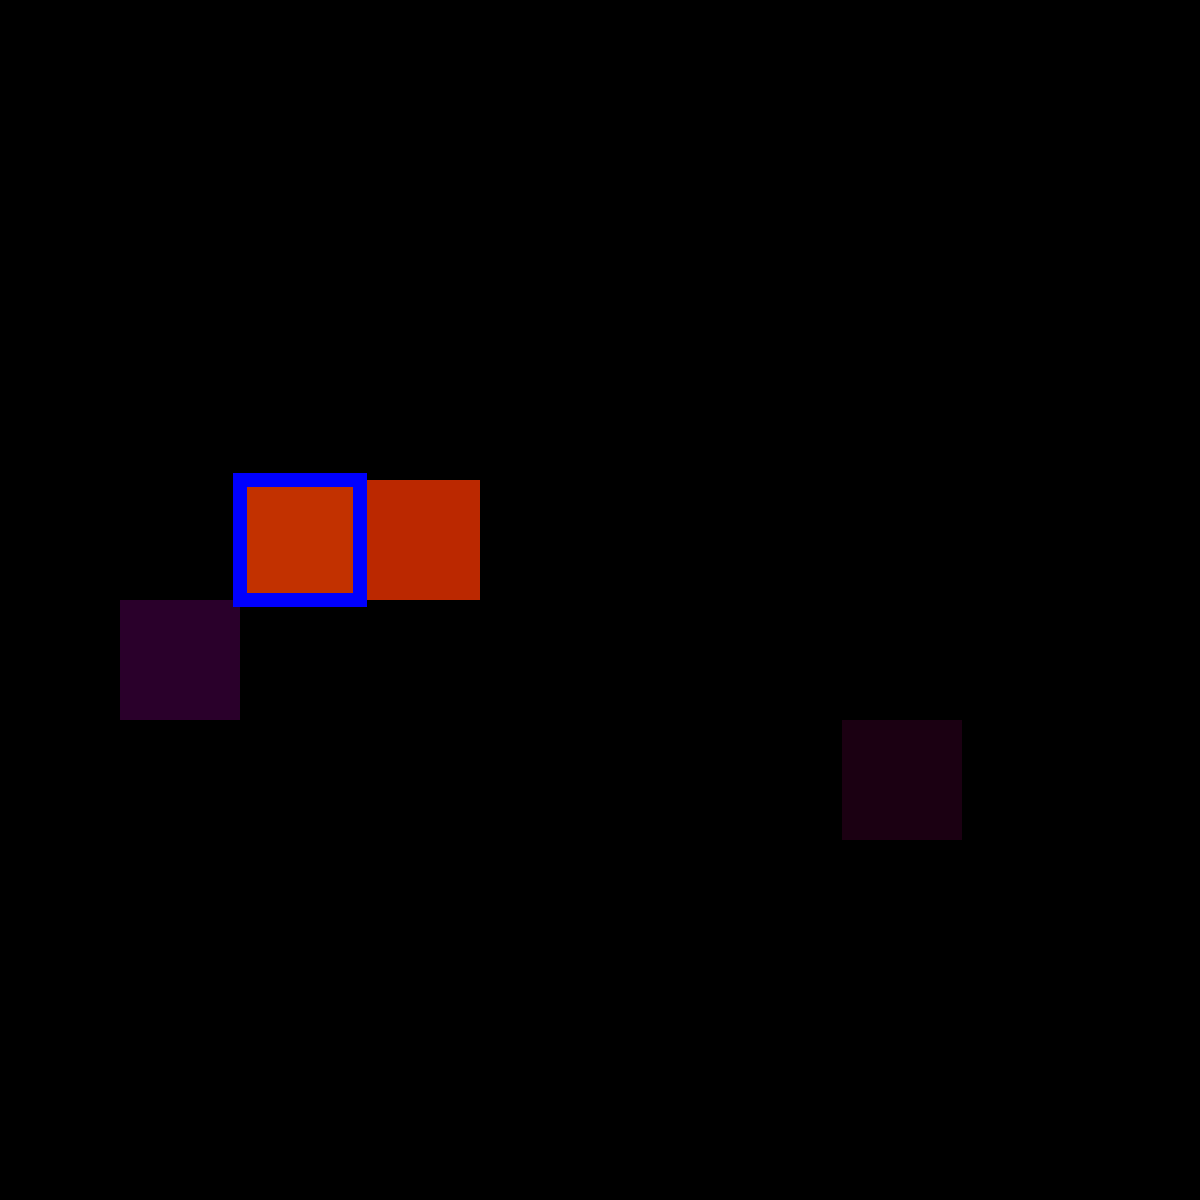
\includegraphics[width=2.4cm]{encoding_1935}};

    \end{tikzpicture}
\end{preview}
\end{document}
